% Replaces the "Further diagrams to include in the final report:" bullet list in Appendix E.
% Figure E.1 (controller state machine) is left unchanged.

\section*{E.2 System Architecture}
Figure~\ref{fig:e-architecture} expands the four-stage architecture of Figure~5.1 into
individual components. Video frames flow through the detector, tracker, state estimator,
priority manager and signal controller to the SUMO adapter. SUMO returns the traffic state
to the state estimator, the recovery manager acts on the controller after preemption, and
all modules exchange events over the FastAPI/MQTT layer and are recorded by the logger.

\begin{figure}[htbp]
  \centering
  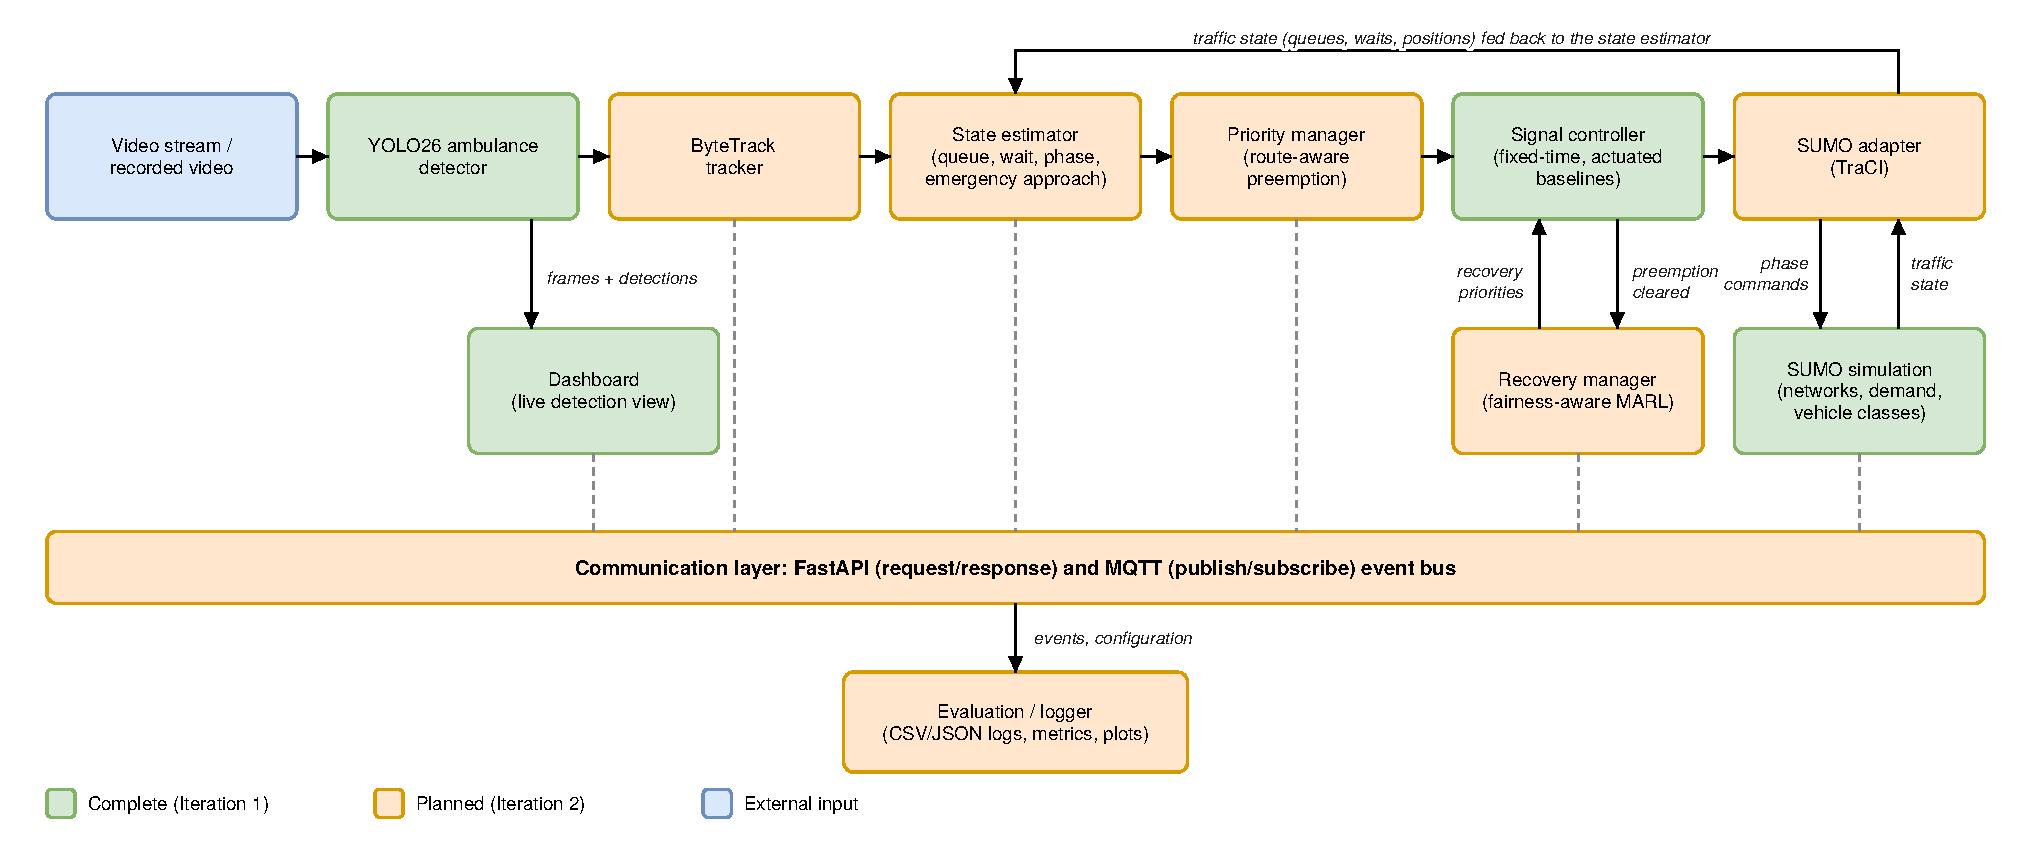
\includegraphics[width=\textwidth]{fig_architecture.pdf}
  \caption{Component-level system architecture (green: complete; orange: Iteration 2).}
  \label{fig:e-architecture}
\end{figure}

\section*{E.3 Activity Diagram}
Figure~\ref{fig:e-activity} shows the activity flow from normal operation through
detection, safe preemption, passage monitoring and recovery back to normal operation,
following the process in Section~5.8.

\begin{figure}[htbp]
  \centering
  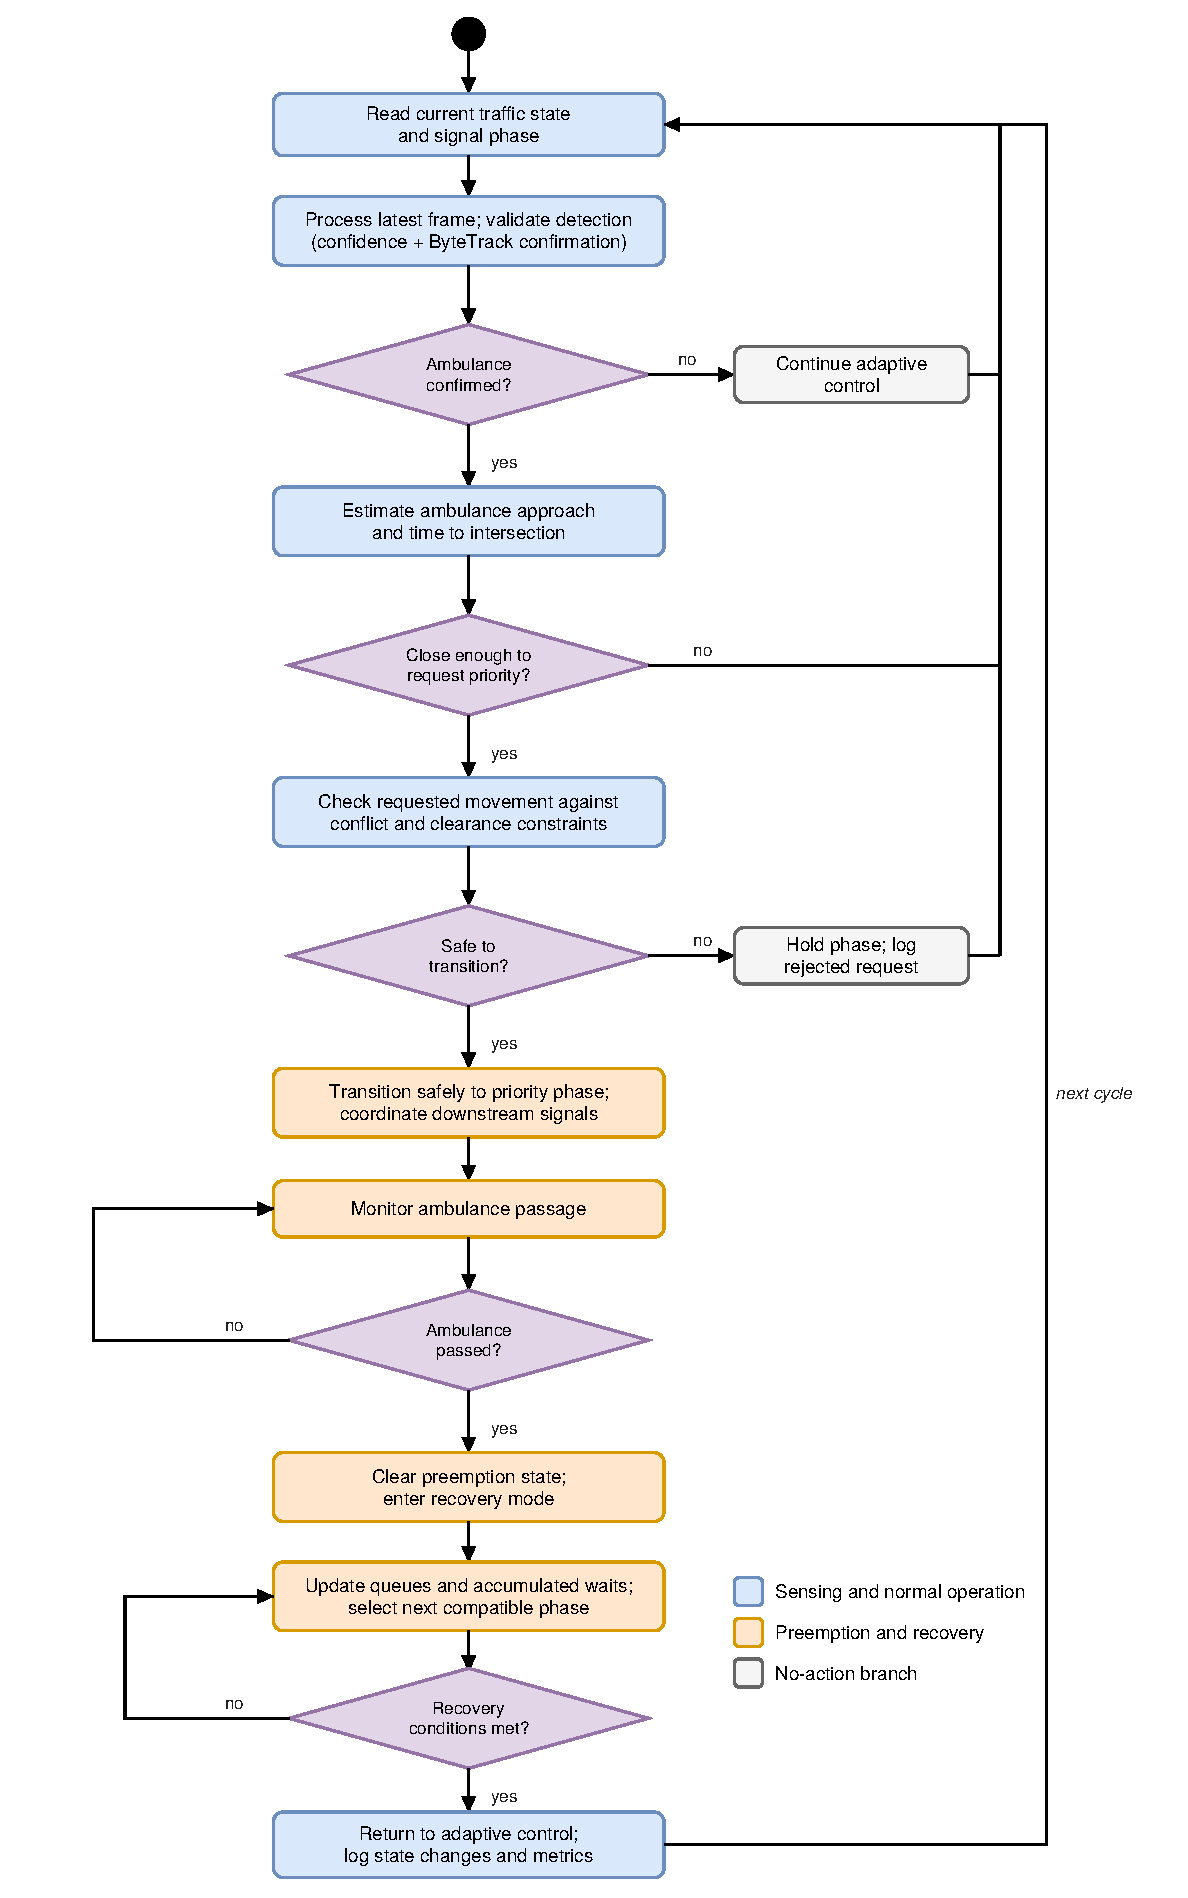
\includegraphics[height=0.85\textheight]{fig_activity.pdf}
  \caption{Activity diagram: detection, safe preemption, passage, recovery and return to normal control.}
  \label{fig:e-activity}
\end{figure}

\section*{E.4 Sequence Diagram}
Figure~\ref{fig:e-sequence} shows the message sequence for an ambulance that passes two
consecutive intersections, including downstream preparation and post-preemption recovery.

\begin{figure}[htbp]
  \centering
  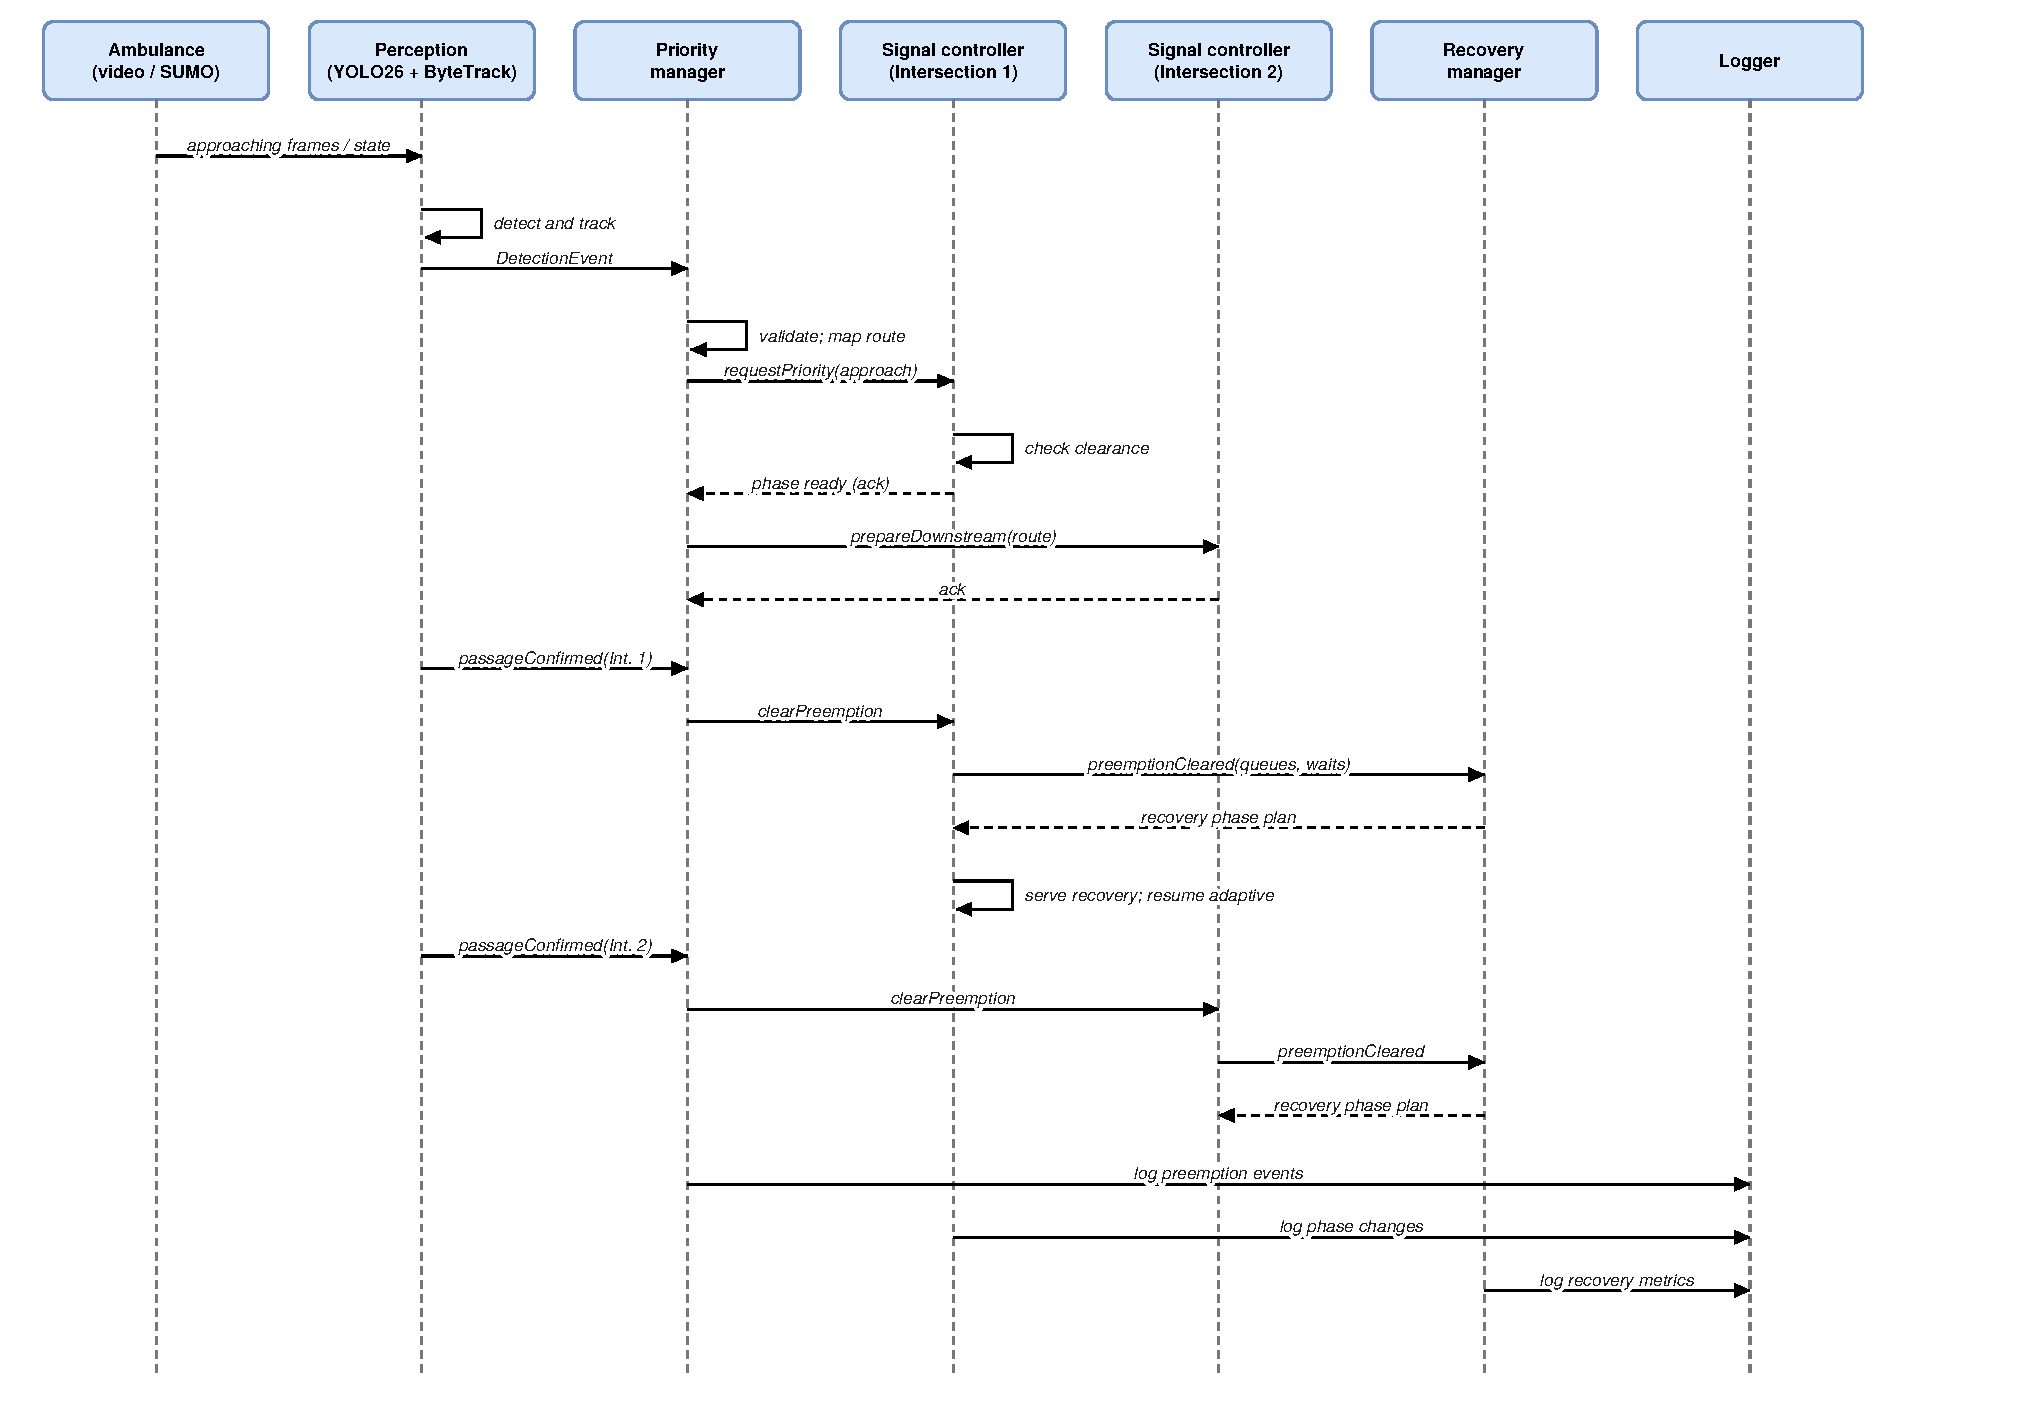
\includegraphics[width=\textwidth]{fig_sequence.pdf}
  \caption{Sequence diagram for an ambulance approaching a sequence of two intersections.}
  \label{fig:e-sequence}
\end{figure}

\section*{E.5 Data-Flow Diagram}
Figure~\ref{fig:e-dfd} shows the level-1 data flow between the external entities
(video source, operator), the six processes, and the three data stores.

\begin{figure}[htbp]
  \centering
  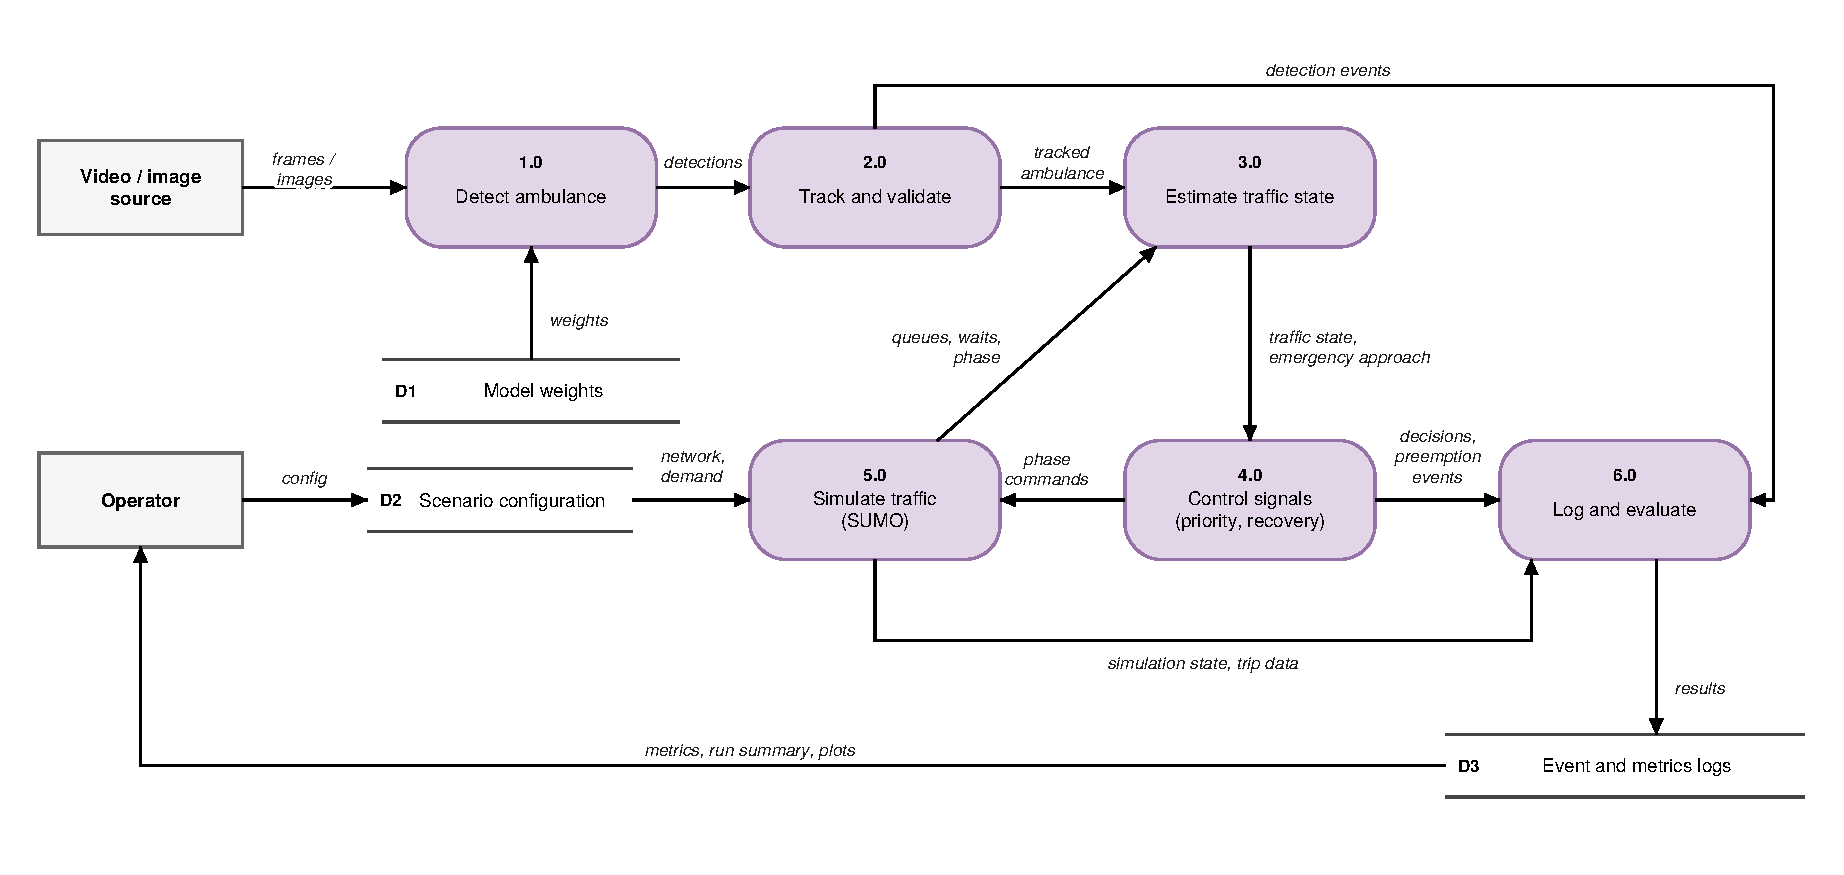
\includegraphics[width=\textwidth]{fig_dfd.pdf}
  \caption{Level-1 data-flow diagram: images, model weights, simulation state, controller actions and metric outputs.}
  \label{fig:e-dfd}
\end{figure}
